\documentclass[tikz]{standalone}

\usepackage{amsmath}
\usepackage{unicode-math}
\usepackage{mathtools}
\usepackage{derivative}

\setmainfont{Stix Two Text}
\setmathfont{Stix Two Math}

\usetikzlibrary{arrows.meta,fit,positioning}

\renewcommand{\familydefault}{\sfdefault}

% prefix equation numbers with section number
\numberwithin{equation}{section}

\DeclarePairedDelimiter{\ceil}{\lceil}{\rceil}
\DeclarePairedDelimiter{\floor}{\lfloor}{\rfloor}
\DeclarePairedDelimiter{\abs}{\lvert}{\rvert}
\DeclarePairedDelimiter{\norm}{\lVert}{\rVert}
\DeclarePairedDelimiter{\bra}{\langle}{\rvert}
\DeclarePairedDelimiter{\ket}{\lvert}{\rangle}
\DeclarePairedDelimiter{\expval}{\langle}{\rangle}
\DeclarePairedDelimiter{\norder}{\mathcolon}{\mathcolon}
\DeclarePairedDelimiter{\anorder}{\typecolon}{\typecolon}
	
\newcommand{\laplace}{\mbfnabla^2}
\newcommand{\trans}{{\scriptscriptstyle\mathsf{T}}}

\newcommand{\vdot}{\cdot}
\newcommand{\vcross}{\vectimes}
\newcommand{\vb}[1]{\symbfup{#1}}
\newcommand{\vu}[1]{\hat{\vb{#1}}}
\newcommand*\dd[2][\relax]{\mathop{\ifx\relax#1\odif{#2}\else \odif[order={#1}]{#2}\fi\,}}

\newcommand{\vacuum}{\ket*{\vb{0}}}

\DeclareMathOperator{\trace}{Tr}
\DeclareMathOperator{\sinc}{sinc}

\AtBeginDocument{
	\let\Re\relax
	\let\Im\relax
	\DeclareMathOperator{\Re}{Re}
	\DeclareMathOperator{\Im}{Im}

	\renewcommand{\div}{\mathop{\mbfnabla\vdot}}
	\newcommand{\curl}{\mathop{\mbfnabla\vectimes}}
}

\DeclarePairedDelimiterX{\comm}[2]{[}{]}{#1,#2}

\DeclarePairedDelimiterX{\braket}[2]{\langle}{\rangle}{#1\delimsize\vert#2}
\DeclarePairedDelimiterX{\ketbra}[1]{\lvert}{\rvert}{#1\rangle\delimsize\langle#1}



\begin{document}
	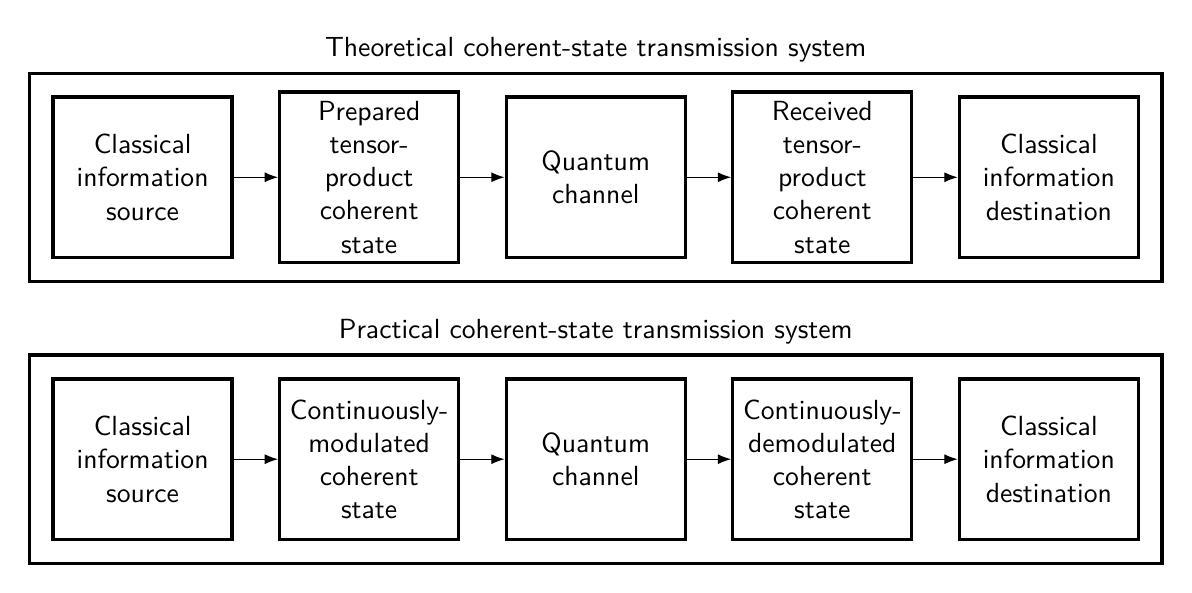
\begin{tikzpicture}[
		node distance=16pt,
		block/.style={draw, very thick, minimum height=58pt, minimum width=58pt, text width=58pt, align=center},
		superblock/.style={draw, very thick, inner sep=8pt},
	]
		\node (theo tx info) [block] {Classical information source};
		\node (theo tx state) [block, right=of theo tx info] {Prepared tensor-product coherent state};
		\node (theo channel) [block, right=of theo tx state] {Quantum channel};
		\node (theo rx state) [block, right=of theo channel] {Received tensor-product coherent state};
		\node (theo rx info) [block, right=of theo rx state] {Classical information destination};
		
		\draw[-Latex] (theo tx info) -- (theo tx state);
		\draw[-Latex] (theo tx state) -- (theo channel);
		\draw[-Latex] (theo channel) -- (theo rx state);
		\draw[-Latex] (theo rx state) -- (theo rx info);
		
		\node [superblock, label={Theoretical coherent-state transmission system}, fit=(theo tx info) (theo rx info)] {};

		\node (prac tx info) [block, below=1.5cm of theo tx info] {Classical information source};
		\node (prac tx state) [block, right=of prac tx info] {Continuously-modulated coherent state};
		\node (prac channel) [block, right=of prac tx state] {Quantum channel};
		\node (prac rx state) [block, right=of prac channel] {Continuously-demodulated coherent state};
		\node (prac rx info) [block, right=of prac rx state] {Classical information destination};
		
		\draw[-Latex] (prac tx info) -- (prac tx state);
		\draw[-Latex] (prac tx state) -- (prac channel);
		\draw[-Latex] (prac channel) -- (prac rx state);
		\draw[-Latex] (prac rx state) -- (prac rx info);
		
		\node [superblock, label={Practical coherent-state transmission system}, fit=(prac tx info) (prac rx info)] {};
	\end{tikzpicture}
\end{document}
